\label{app:poisoning}

\paragraph{Calibration time label flipping attacks} Most conformal score functions are often not Lipschitz continuous with respect to $y \in \labelspace$. Therefore we devise no straightforward certificate for label flipping attacks. However, the defense to label flipping attacks defined in \cite{cas} that leverages the computation of a maximum quantile shift when scores are permuted is valid for our networks too.

\paragraph{Calibration time feature poisoning attacks} In the context of calibration-time feature poisoning however the Lipschitz condition of our score with respect to $x \in \inputspace$ becomes greatly advantageous. Indeed, the problem of computing the maximum quantile shift becomes simplified in the sense that every score verifies a $L_s$ Lipschitz condition and is interdependent from the scores of other calibration samples for the true class. We devise a simple Linear Programming script described in Figure~\ref{fig:poisoning_quick} to handle the computation of the maximum and minimum quantile shift under attack of budget $(k,\epsilon)$. We verify our Linear Programming solution empirically on the \emph{CIFAR-10} dataset (see Table \ref{tab:featurepoisoning}). 

\paragraph{NB} Importantly, our algorithm assumes that the quantile computation done during the calibration step returns $\calthreshold=\overrightarrow{R}_{\lceil (n+1)(1-\alpha)\rceil}$.


\begin{table}[h!]
  \centering
  \small
  \sisetup{
    detect-weight=true,
    detect-family=true,
    table-number-alignment = center,
    table-format=1.4
  }
  \begin{tabular}{
      S[table-format=1.2] 
      S[table-format=2.0] 
      l 
      S 
      S
    }
    \toprule
    {\(\epsilon\)} & {k} & {Metric} & {Mean} & {Std Dev} \\
    \midrule
    0     & {--} & Val.\ accuracy           & 0.7260 & {--}    \\
          &      & Set size                 & 2.0690 & 0.0387  \\
    0.25  & 6    & Robust CP \(\gamma\)     & 0.8982 & 0.0085  \\
          &      & Robust CP set size       & 2.0699 & 0.0467  \\
    0.25  & 50   & Robust CP \(\gamma\)     & 0.9090 & 0.0068  \\
          &      & Robust CP set size       & 2.1872 & 0.0466  \\
    \bottomrule
  \end{tabular}
  \caption{Summary of empirical coverage and prediction set sizes across different attack budgets \((k,\epsilon)\) for feature poisoning on the calibration set (\(n_{cal}=4750\)). Each experiment was repeated 10 times with a randomly selected calibration subset.}
  \label{tab:featurepoisoning}
\end{table}

\begin{figure}[h!]
    \centering
    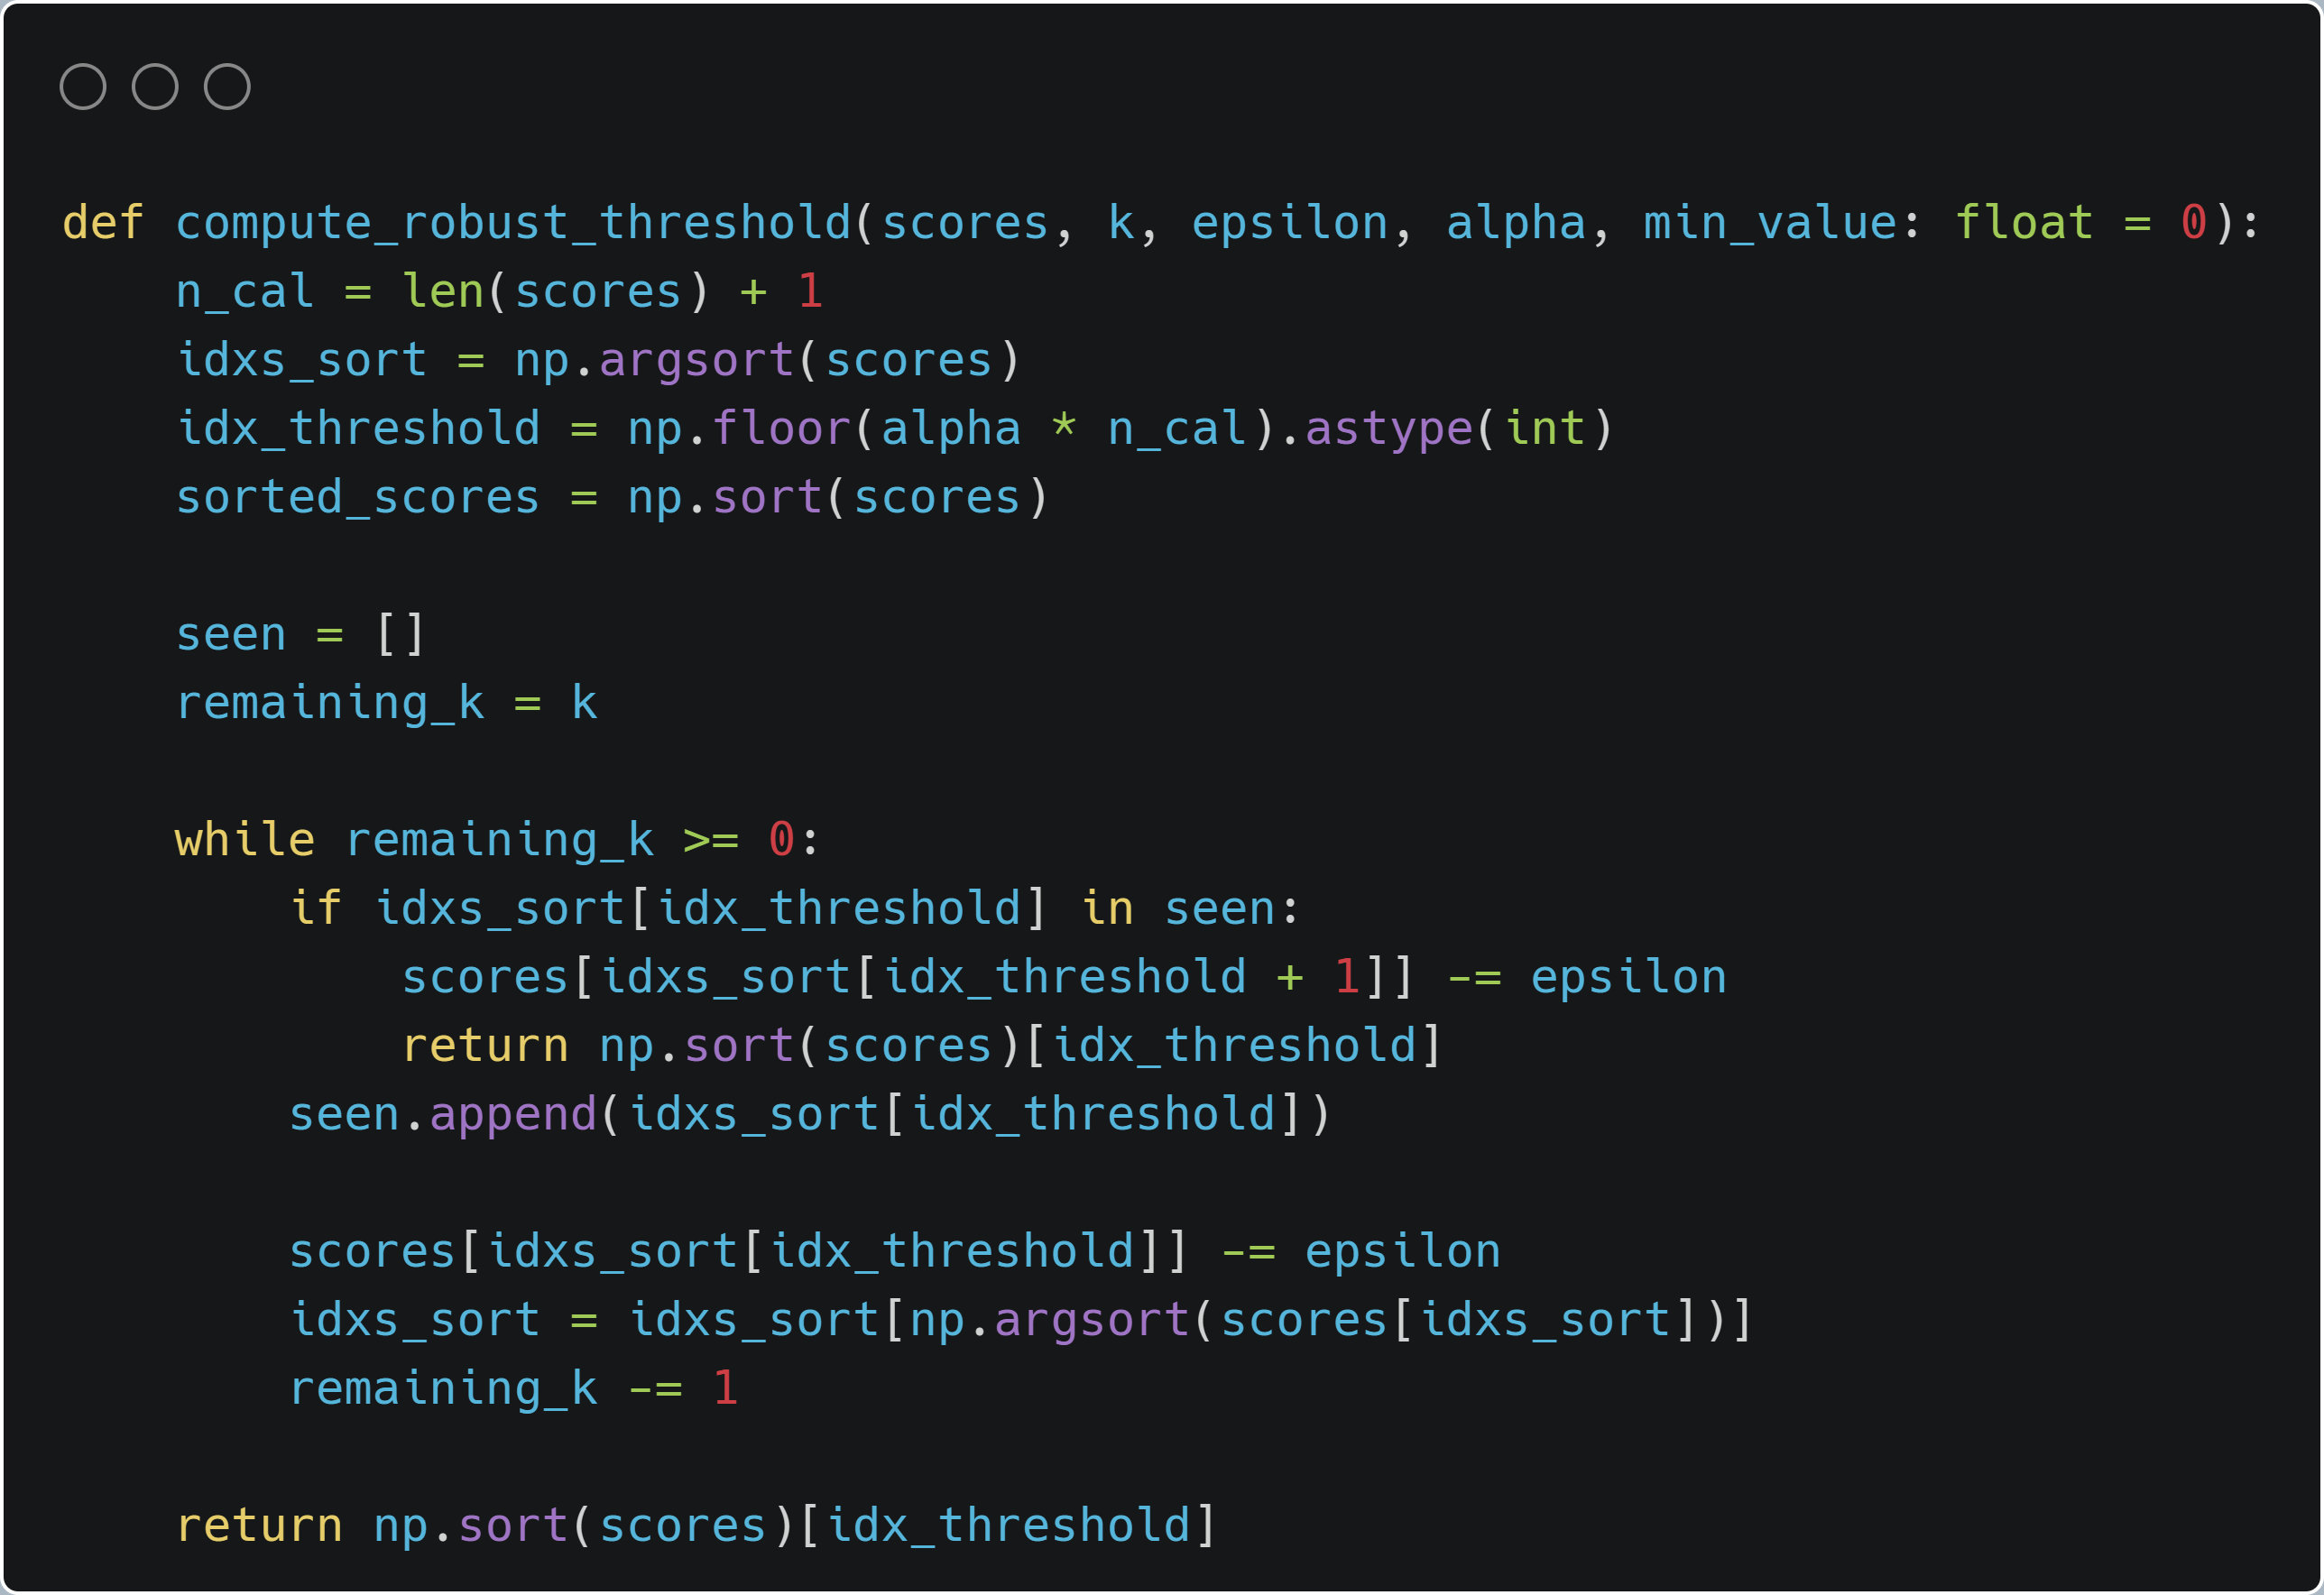
\includegraphics[width=0.5\linewidth]{poisoning_carbon.png}
    \caption{Our function for computing the maximum quantile shift and therefore certifying the robustness of prediction sets under calibration time feature poisoning attacks.}
    \label{fig:poisoning_quick}
\end{figure}
